
\documentclass[10pt,twocolumn,letterpaper]{article}

\usepackage{cvpr}
\usepackage{url}
\usepackage{times}
\usepackage{epsfig}
\usepackage{graphicx}
\usepackage{amsmath}
\usepackage{amssymb}
\usepackage{lipsum}
\usepackage{midfloat}
\DeclareUnicodeCharacter{2212}{-}
%\documentclass{article}
\usepackage{graphicx}
\graphicspath{ {./images/} }

% Include other packages here, before hyperref.

% If you comment hyperref and then uncomment it, you should delete
% egpaper.aux before re-running latex.  (Or just hit 'q' on the first latex
% run, let it finish, and you should be clear).
\usepackage[breaklinks=true,bookmarks=false]{hyperref}

\cvprfinalcopy % *** Uncomment this line for the final submission

\def\cvprPaperID{****} % *** Enter the CVPR Paper ID here
\def\httilde{\mbox{\tt\raisebox{-.5ex}{\symbol{126}}}}

% Pages are numbered in submission mode, and unnumbered in camera-ready
%\ifcvprfinal\pagestyle{empty}\fi
\setcounter{page}{4321}
\begin{document}

%%%%%%%%% TITLE
\title{Image Colorization using GAN and Inception-ResNet-v2}

\author{Olivia Beyer Bruvik\\
Stanford University\\
% Institution1 address\\
{\tt\small oliviabb@stanford.edu}
% For a paper whose authors are all at the same institution,
% omit the following lines up until the closing ``}''.
% Additional authors and addresses can be added with ``\and'',
% just like the second author.
% To save space, use either the email address or home page, not both
\and
Mia Penfold\\
Stanford University\\
% First line of institution2 address\\
{\tt\small penfold@stanford.edu}
}

\maketitle
%\thispagestyle{empty}

%%%%%%%%% ABSTRACT
\begin{abstract}
   In this paper, we propose a novel generative adversarial network (GAN) based model for image colorization. Our model incorporates semantic features extracted from a pre-trained Inception-ResNet-v2 model to enhance the realism of the colorized images. We compare our approach to two baseline models: a convolutional neural network (CNN) based model with semantic feature extraction (Deep Koalarization by Baldassarre et al.) and a conditional GAN model (pix2pix by Isola et al.) ~\cite{Koalarization, Pix2Pix}. Our experimental results demonstrate that our proposed method achieves strong performance in terms of both quantitative metrics (PSNR and SSIM) and visual quality.
\end{abstract}

\section{Introduction}
Image colorization is the process of assigning color values to each pixel of a grayscale image to obtain a colorized version. Colorized images provide a better visual representation of reality. The ability to give color to grayscale images is therefore a highly desirable application of computer vision. It has applications in the movie animation industry, allows for efficient compression of security footage, and it has also been used to colorize historical photographs~\cite{Huang}.  Image colorization is a multi-modal problem: one target can have multiple appropriate colors. A T-shirt, for example, can be reasonably be colored blue, red or virtually any color. The task to give a computer a black and white image and produce a plausible colorization that could potentially fool a human observer remains and interesting and complex problem as well as an ongoing area of research.

For this project, we seek to develop a model that can colorize black and white images in a way that is realistic to the human eye. We will do so by building a generative adverserial network (GAN) that incorporates semantic features. We will use the Inception-ResNet-v2 with pretrained weights to extract high-level semantic features, and incorporate those features into a U-Net generator. We will do this with the purpose of enhancing existing colorization techniques.

The input to our algorithm is a 1-channel grayscale image. We then use our GAN model to output a predicted colored image with 3-channels. 

\section{Related Works}
Several approaches to colorizing black and white images have been proposed across the years, including the use of convolutional neural networks (CNNs), generative adversarial networks (GANs), and transformers~\cite{Huang}.

Colorization models learn prediction functions from large datasets of color images at training time, posing the problem as either regression onto continuous color space~\cite{Zhang} or classification of individual pixels into quantized color values  which are then trained to minimize the error between the output and the ground truth~\cite{Koalarization}.

\subsection{Convolutional Neural Networks}
CNN-based colorization models frame the colorization problem as a classification task~\cite{Zhang}. They use a Euclidian (L2) loss to label each pixel in a grayscale image (L) to its corresponding color values (a, b) labels~\cite{Cheng, Zhang}.

CNNs with a naive pixel-wise loss function of this kind show moderate success. Although this method performs well for natural image colorization, its application is largely limited by the need to use reference images \cite{Huang}. Additionally, the loss is not robust to the multimodal nature of the colorization problem, these models tend to assign only one color to the same object, whereas in practice there are multiple potential colors~\cite{Zhang}. Models with these types of loss functions will generate blurry, grayish results and bland outputs in an effort to minimize the Euclidean distance between the predicted and ground truth pixel value~\cite{Pix2Pix}.

CNN-based colorization methods usually require a large-scale  dataset of reference images to train the learning model to realize image colorization. However, it is difficult to obtain the image dataset containing all the objects to train the neural network model in the actual training process, which greatly limits the performance of this method~\cite{Huang}. 

\subsection{Generative Adversarial Networks}
GANs, first proposed in 2014~\cite{Goodfellow}, show promising results in addressing multimodal problems.  GANs consist of two neural networks—a generator and a discriminator—trained adversarially. The generator network takes in random noise as input and trains to create outputs that cannot be distinguished from “real” outputs by the adversarially trained discriminator. The discriminator is trained to detect the generator’s “fakes” as best it can. This adversarial training allows the generator to learn and produce increasingly realistic data samples.

Generative models such as conditional GANs have thus entered the field as a general-purpose solution to image-to-image translation and that is particularly suitable for image colorization~\cite{Huang, Zhang}. Instead of generating images from random noise, conditional GANs are given a condition to generate an output image~\cite{Mirza}.  In colorization models, the grayscale image is the condition for colorization. Pix2Pix is a conditional-GAN that exclusively takes images as the condition~\cite{Pix2Pix}. It is a widely used model used to adress image-to-image translation problem like colorization ~\cite{Zhao}. This seminal paper not only motivated us to adopt a cGAN approach for our model but also provided valuable insights for our implementation.

GAN-based colorization models generally produced results that were more vibrant and lifelike outcomes compared to convolutional neural networks (CNNs)~\cite{Pix2Pix}.

\subsection{Incorporating Semantic Meaning into CNN}
Several papers noted that extracting semantic information from the models input could be valuable in producing more realistic outputs~\cite{Zhang, Pix2Pix}. The semantics of the scene and its surface texture can provide ample cues for how to colorize different regions of an image. Grass is typically green, the sky is typically blue, and tree trunks are always brown. Even in cases where many possible colors exist, an object semantics can provide some guidance: cars can be white, blue, red and many other colors, but they are seldom pink or orange.  Baldassarre et al. created a model that uses explicit semantic feature extraction to insert into the model~\cite{Koalarization}. Their approach involves fusing the Inception embedding with the output of the convolutional layers of the encoder, effectively inserting these embeddings in the center of the U-Net structure. Their model was often able to produce convincing results, but still struggled to color objects with a wider range of acceptable colorings, and assigned these grayish tones~\cite{Koalarization}.

\section{Problem Statement}
The goal for this project is to generate realistic colorization of black and white images to the human eye. We aim to do so by developing a a GAN model that also incorporates semantic features by combining a deep convolution neural network. 

We will train this model from scratch with high-level features extracted from the Inception-ResNet-v2 pre-trained model. Our generator will be based on the model outlined by Baldassarre et al., the "Deep Koalarization" model~\cite{Koalarization}, which employs CNNs and Inception-ResNet-v2. 

To our knowledge, the combination of a generative adverserial network with semantic feature extraction via the Inception-ResNet-v2 has not been implemented for the purpose of colorization before. We aim to implement such a model with the purpose of improving the realism of colorization. 

% the Deep Koalarization model~\cite{Authors14} developed by Baldassarre et al., which employs CNNs and Inception-ResNet-v2. Their model combines a deep Convolutional Neural Network trained from scratch with high-level features extracted from the Inception-ResNet-v2 pre-trained model. 

% Baldassarre et al. utilize a Euclidean distance loss function that measures the Mean Square Error (MSE) between the predicted pixel colors and the target colors. While this is a common loss function for colorization, it leads to two major issues of brown-ish tones and blurry features. This occurs because the Euclidean distance is minimized by averaging all plausible outputs, which causes blurry results~\cite{Authors15} and conservative colorization. 

%%%%%%%%% BODY TEXT
\section{Data and Features}
\subsection{COCO Dataset}
We will train this model on the COCO dataset. The COCO (Common Objects in Context) dataset is a large-scale dataset containing  330,000 images with annotations for object detection, segmentation, and captioning. It is widely used for training and evaluating computer vision models, particularly in object detection, segmentation, and captioning tasks. The dataset includes over 1.5 million object instances across 80 object categories and each image has 5 different captions describing the scene.

\subsection{Inception-ResNet-v2}
Inception-ResNet-v2 is a deep convolutional neural network architecture that combines the Inception network with residual connections, replacing the filter concatenation stage of the Inception architecture first proposed by researchers at Google in 2016. The network is pre-trained on the ImageNet dataset, allowing it to classify images into 1000 object categories. Inception-ResNet-v2 can be used for various computer vision tasks, such as image classification, object detection, and transfer learning.

\subsection{DeepLabV3-ResNet50}
DeepLabV3-ResNet50 is a fully concolutional neural network designed for semantic segmentation. It uses pre-trained ResNet models as the backbone feature extractor,  as well as the Atrous Spatial Pyramid Pooling (ASPP) module to robustly segment objects at multiple scales. DeepLabV3-ResNet50 also uses dilated convolutions to capture multi-scale information and control the resolution of feature maps. DeepLabV3-ResNet50 model we are using is trained on a subset of COCO, using only the 20 categories that are present in the Pascal VOC dataset.

\subsection{Data Pre-processing}
In order to train the GAN model on our images to follow this mapping we preprocess the data as follows: we resize the images to be of width and height \(256 \times 256\); perform a random horizontal flip on training images as a way of augmenting the data; convert each RGB image into Lab color space; generate training data in the form of pairs of images \(\{L, ab\}\), where \(L\) and \(ab\) are two different depictions of the same underlying scene; \(L\) is the grayscale version of the image and \(ab\) are the two corresponding color channels; convert \(L\) to [\(-1,1\)]; convert \(a, b\) to [\(-1,1\)].

\subsection{CIE L*a*b* Color Cpace}
The images in the datasets are RGB. However, The colorization problem is generally posed in the CIE L*a*b* color space. In this colorspace, grayscale images can be represented using a singular channel, the channel L. Meanwhile, RGB requires all three of its channels to represent the image in color and in grayscale. A colorization model in the CIE L*a*b* color space, converts an input \(X_L \in R_{H\times W\times 1}\) into an output \(X_L \in R_{H \times W\times 3}\)  creating a mapping \(F\) such that \(F:X_L \rightarrow (X_a,X_b)\) allowing the colorization problem to be posed as a one-to-two mapping as opposed to three-to-three. 

\section{Methods}
For this project, we aim to improve the quality of colorization of black and white images. We will develop a cGAN based on the pix2pix model. We will edit the generator structure to incorporate semantic meaning based on the model created by Baldassare et al.~\cite{Koalarization}, which combines a CNN with the Inception-ResNet-v2 pre-trained model (Figure 1). We will use Baldassare et al.'s "Deep Koalarization" model as a baseline model with which to compare our results~\cite{Koalarization}. 

\subsection{Baseline method #1: "Deep Koalarization" by Baldassare et al.}

%The model created by Baldassarre et al. inserts explicit semantic feature into their model by combining a deep Convolutional Neural Network U-Net trained from scratch with high-level features extracted from the Inception-ResNet-v2 pre-trained model. 
%The approach taken by Baldassarre et al. highlighted the effectiveness of feeding semantic information to a colorization model and informed the choice of the Inception-ResNet-v2 pre-trained model as the feature extractor to incorporate into our model. Its difficulty avoiding greyish output similarly sparked interest in exploring whether similar semantic segmentation could enhance the colorfulness of results in a GAN, which tend to have more colorful outputs that CNNs.  Their technical implementation of the fusion has also informed the way we envision incorporating semantic meaning into our GAN generator.
The model created by Baldassarre et al. inserts explicit semantic feature into their model by combining a deep Convolutional Neural Network trained from scratch with high-level features extracted from the Inception-ResNet-v2 pre- trained model. It is a U-Net generator with an Inception-ResNet-v2 fused into the layer between the encoder and decoder (Figure 1).

They find the optimal model parameters by minimizing an objective function defined over the estimated output and the target output. To quantify the model loss, Mean Square Error is employed between the estimated pixel colors in a*b* space and their real value. For a picture X, MSE is calculated as described in equation (1). 

\begin{equation}
C(\mathbf{X}, \boldsymbol{\theta})=\frac{1}{2 H W} \sum_{k \in\{a, b\}} \sum_{i=1}^H \sum_{j=1}^W\left(X_{k_{i, j}}-\tilde{X}_{k_{i, j}}\right)^2
\end{equation}

\(\theta\) represents all model parameters, \(X_{ki,j}\) and \(\widetilde{X}_{ki,j}\) denote the \(i,j\)-th pixel value of the \(k\)-th component of the target and reconstructed image, respectively. This can easily be extended to a batch \(B\) by averaging the cost among all images in the batch, i.e. \(\frac{1}{|B|} \sum_{X \in B} C(X, \theta)\).

While training, this loss is backpropagated to update the model parameters \(\theta\) using Adam Optimizer \cite{Kingma} with an initial learning rate \(\eta = 0.001\). During training, they impose a fixed input image size to allow for batch processing.

\begin{figure}
    \centering
    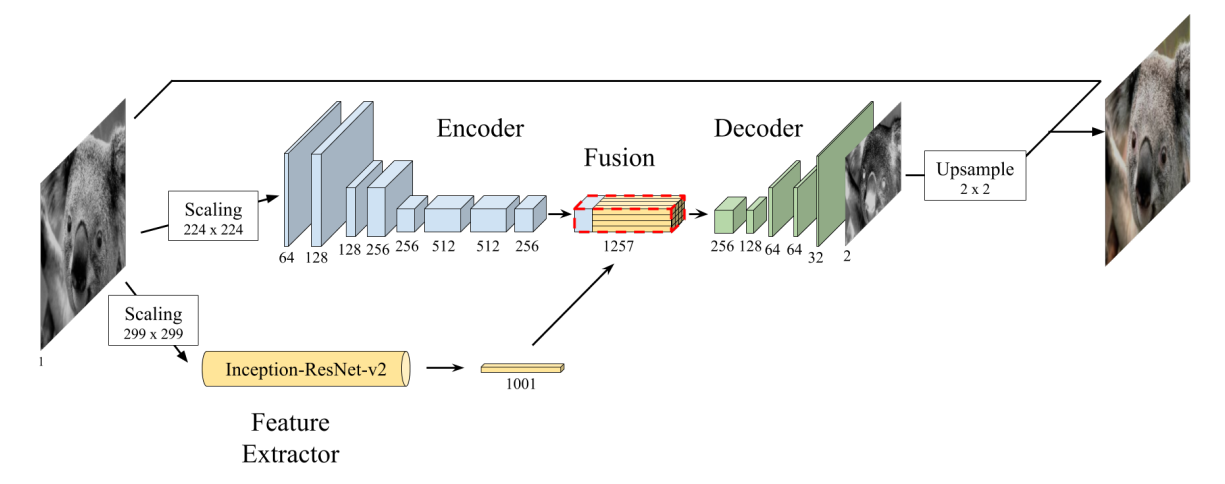
\includegraphics[scale=0.2]{baldassare_model.png}
    \caption{An overview of the generator network architecture}
    \label{fig:enter-label}
\end{figure}


Their model was often able to produce convincing results, but still struggled to color objects with a wider range of acceptable colorings, assigning these grayish tones. The models success-cases showed that semantic information can be a useful addition to colorization models as suggested by literature~\cite{Zhang, Pix2Pix}. Its often bland outputs and underperformance in coloring objects with multiple possible colorings inspired our research to see whether an adversarially trained model would fare better. This paper informed our decision to choose the Inception-ResNet-v2 pre-trained model as a feature extractor to incorporate into our model, its technical implementation of the fusion has also informed the way we envision incorporating semantic meaning into our GAN generator. Baldassare et al.'s model will serve as the baseline against which we compare our results.

\subsection{Baseline method #2: pix2pix by Isola et al.}
Isola et al.'s seminal pix2pix model paper is widely used in generative image-to-image tasks~\cite{Huang}. It is particularly popular because it is not application specific, and is therefore well suited for a variety of tasks~\cite{Pix2Pix}. pix2pix is a conditional GAN that uses a skip-connections generator with a “U-Net" based architecture and a convolutional PatchGAN classifier as a discriminator~\cite{Pix2Pix}. It uses concatenated skip connections to pass on low-level information between the input and output in the generator. The PatchGan descriminator only penalizes structure at the scale of patches
We will be adapting the general-application pix2pix model and adapt it to our colorization task, incorporating into it our generator with embedded semantic information. The model uses an adversarial loss which can be expressed as:
 \begin{equation}
 \begin{split}
\textit{L}_c_G_A_N (G, D) =E_x_,_y [log 
\textit{D(x, y)}] + \\
E_{x, z} [log(1  \textit{D(x, G(x, z))}]
 \end{split}
 \end{equation}

The model additionally utilizes an L1 loss, to also train the model to minimize distance from the ground truth:
 \begin{equation}
 \textit{L}_{L_1}(G) = E_{x, y} [\mid\mid y-G(x,z)\mid\mid_1
 ] \end{equation}

 The final objective of the pix2pix model, to minimize the sum of the two losses, can be defined as follows:
 \begin{equation}
 G = \text{arg}\ \min_{G} \max_{D}\ L_{cGAN(G, D)} + L_{L_1}(G)
 \end{equation}

\subsection{Our method: Inception-GAN Architecture}
In the above section, we detailed the architecture of the GAN for our baseline model. This section will delve into the specifics of the model we developed, comprised of a 1) U-Net generator with an Inception-ResNet-v2 fused into the layer between the encoder and decoder 2) a PatchGAN descriminator.

\begin{table}[]
    \centering
    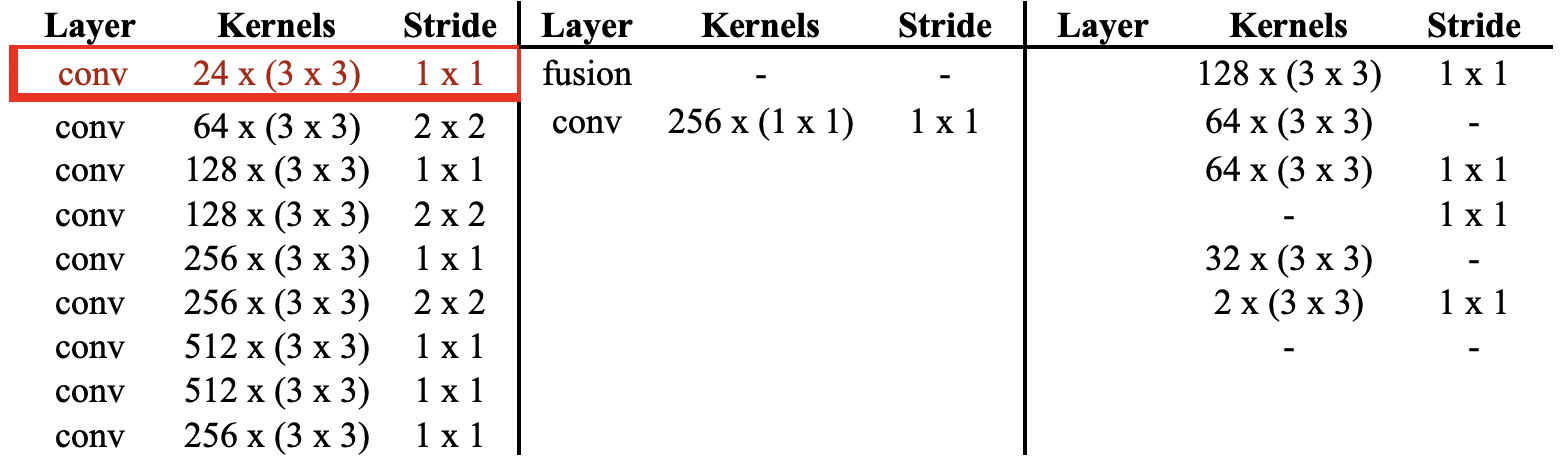
\includegraphics[width=1\linewidth]{layers.png}
    \caption{A summary of the network structure for the generator, influenced by Baldassare et al. LEFT: the encoder network, MIDDLE: fusion network, RIGHT: decoder network. Each convolutional layer utilizes a ReLu activation function, except for the final layer which utilizes a hyperbolic tangent function. The feature extraction branch mirrors the architecture of Inception-Resnet-v2, excluding the last softmax layer. Our model's additional layer is highlighted in red.}
    \label{tab:my_label}
\end{table}

\subsubsection{Architecture of the Generator Network}
 The generator comprises four primary elements: an encoder, a decoder, a fusion layer, and a high-level feature extractor. For the latter, we've opted for the Inception-ResNet-v2 model, leveraging pretrained weights trained on the ImageNet dataset (Figure 1). 

  
\subsubsection{Encoder}
After data is preprocessed, the Encoder processes grayscale images of dimension \(H \times W\). It outputs a H/8 × W/8 × 512 feature representation. In order to do this, it utilizes 9 convolutional layers with \(3 \times 3\) kernels. The encoder uses padding to preserve the layer’s input size. Before the first layer,  it resizes the images to \(256 \times 256\) pixels and stack three of them to get three channels, it subsequently integrates integrated the COCO ResNet model, which contains 21 classes to produce a tensor of dimensions \(24 \times 256 \times 256\). Layers number 2, 4 and 6 apply a stride of 2, which halves the dimension of their output and decreases the number of required computations. The addition of the COCO ResNet model at the beginning of the network and the first \(24 \times 3 \times 3\) convolutional layer is original to this model (see Table 1).

\subsubsection{Feature Extractor} 
Higher-level features, such as "outdoor scenery" or "night-time setting," provide valuable image details utilized during the colorization procedure. To derive an image embedding, we utilized a pre-trained Inception-ResNet-v2 model. The feature extractor resizes the images to \(299 \times 299\) pixels and stack three of them to get three channels as input to the Inception model. The modified image is fed into the network and the output from the final layer preceding the softmax function is retrieved. This process yields a \(1001\times1\times1\) embedding.
 

\subsubsection{Fusion}
The fusion layer integrates the feature vector extracted by Inception by replicating it \(HW/8^2\) times and appending it to the feature volume produced by the encoder along the depth axis (Fig. 3). This results in a unified volume containing both the encoded image and mid-level features, with a shape of \(H/8\times W/8\times 1257\). This repetition and fusion across the volume of the encoder output ensures a uniform distribution of the semantic information across all spatial regions of the image. Finally, we apply 256 convolutional kernels with dimensions of 1×1, yielding a feature volume of \(H/8\times H/8\times 256\).
\subsubsection{Decoder} 
Ultimately, the decoder processes this \(H/8\times H/8\times 256\) volume through a sequence of convolutional and up-sampling layers to yield a final layer measuring \(H\times W\times 2\) in dimensions. Up-sampling is achieved using a straightforward nearest neighbor approach, effectively doubling the height and width of the output compared to the input.

 
\subsection{PatchGAN (Markovian) discriminator}
To model high-frequencies, we use a discriminator architecture called PatchGAN or Markovian Discriminator that only penalizes structure at the scale of patches. The discriminator attempts to classify each patch as real or fake. It operates convolutionally across the image, aggregating responses to produce the final output of D. The discriminator treats the image as a Markov random field, assuming independence between pixels separated by more than a patch diameter. While L1 and L2 loss tend to produce blurry results in image generation problems~\cite{Larsen} and generally fail to produce high-frequency sharpness, they do often capture low frequencies accurately. This is why the GAN discriminator focuses on solely represent high-frequency patterns, depending on an L1 term to ensure accuracy in low-frequency components (Eqn. 4). 

\subsection{Pretraining the generator}
Inspired by Youssef~\cite{Youssef} and Ledig et al.~\cite{Ledig}, we chose to separately pretrain the generator in a supervised and deterministic way. We did this to avoid the problem of "the blind leading the blind" that can occur in GANs, where at when training starts, neither generator nor discriminator have learnt to do their tasks well. The generator is pretrained with L1 loss to colorize images. It is trained for 20 epochs with a learning rate of 1e-4.

\subsection{Optimization}
To optimize our networks we alternate training D, and G. As suggested in the original GAN paper G is trained to maximize log D(x, G(x, z)) instead of to minimize log(1 − D(x, G(x, z)). For every 5 gradient descent steps that G takes, D takes one. This is meant to slow down the rate at which D learns relative to G. We train on 10,000 randomly chosen images (training = 8,000, validation = 2,000) for 15 epochs and use minibatch SGD using the  Adam optimization algorithm, with a learning rate of 2e-4 for both the generator and the discriminator, and momentum parameters β1 = 0.5, β2 = 0.999.
\begin{figure}
    \centering
    \includegraphics[width=0.5\linewidth]{Screenshot 2024-06-05 at 9.37.09 AM.png}
    \caption{Results from Batch 16 training on test set}
    \label{fig:enter-label}
\end{figure}

\begin{figure}
    \centering
    \includegraphics[width=1\linewidth]{Screenshot 2024-06-05 at 6.43.49 PM.png}
    \caption{Training loss. Discriminator training faster than GAN before changes}
    \label{fig:enter-label}
\end{figure}
\subsection{Experiments}
During training, we noticed the discriminator outpaced the generator. We attempted to change the learning rate but found this to be ineffective, likely because we used the Adam optimizer which is a self-tuning algorithm ~\cite{Kingma}. Because of this, we retained Baldassare et al.'s recommended rates (2e-4 learning rate, betas of 0.5 and 0.999) for both generator and discriminator and slowed the discriminator by altering the frequency of discriminator updates relative to the generator. Updating the discriminator once for every five generator updates yielded optimal results. Batch sizes of 16 and 64 were tested for pre-training and training, with 64 proving most effective. The original pix2pix model, which uses noise via dropout layers in the generator architecture~\cite{Pix2Pix}. We trained the model with dropout layers with probability 0.2 and 0.5 and with no dropout and ultimately found that the model worked best without dropout. Recent research by the author suggests dropout isn't essential for colorization models. They noted the grayscale input still provides ample information for the generator to produce compelling results, but that the outputs are more deterministic~\cite{Pix2Pix, Shariatnia}. We also experimented with adding concatenating information from DeepLabV3 trained on COCO before an initial convolutional, which seemed to help with color droplets on the produced images.

\begin{figure}
    \centering
    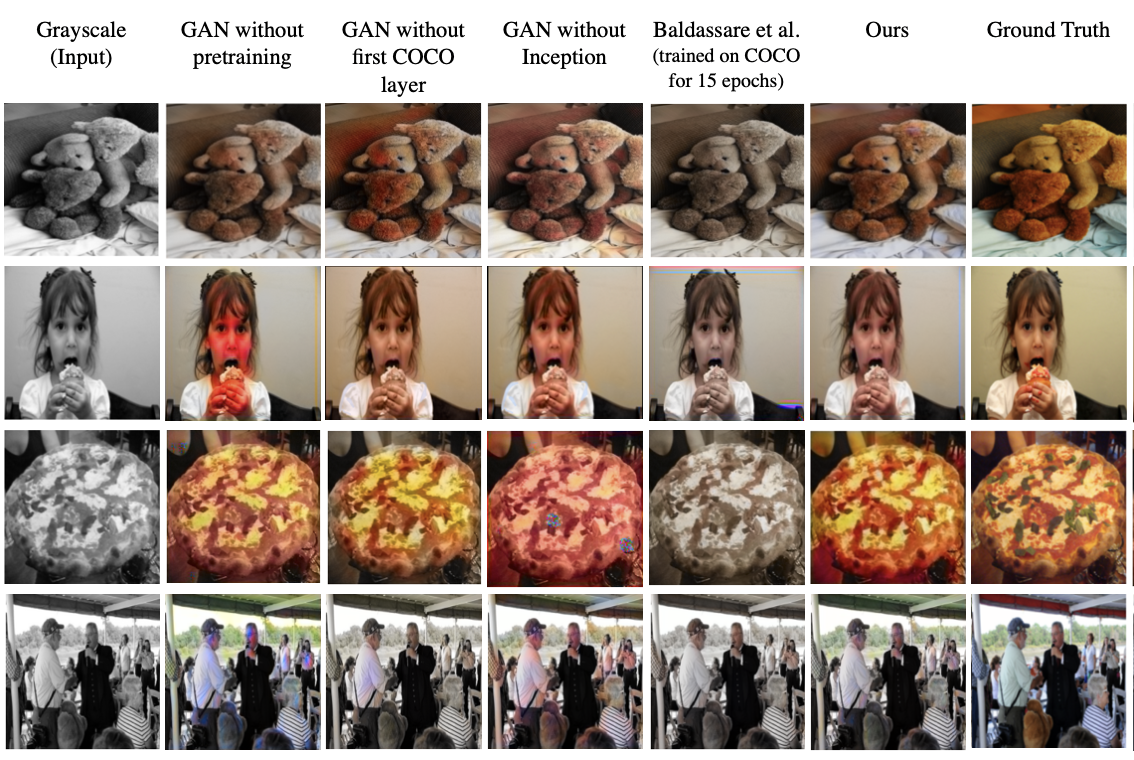
\includegraphics[width=1\linewidth]{latex/results_final.png}
    \caption{Ablation studies and comparison to baseline on test-set (64 batches and trained for 15 epochs on 10,000 COCO images)}
    \label{fig:enter-label}
\end{figure}
\section{Discussion}
\begin{table}
    \centering
    \includegraphics[width=1\linewidth]{Screenshot 2024-06-05 at 7.50.32 PM.png}
    \caption{PSNR and channel-wise SSIM for ablation studies and comparison to baseline}
    \label{fig:enter-label}
\end{table}
\begin{table}
    \centering
    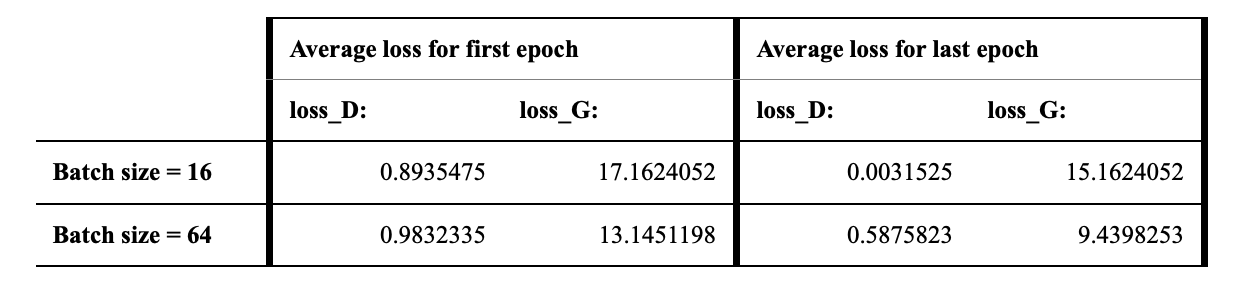
\includegraphics[width=1\linewidth]{latex/loss for batches.png}
    \caption{Losses for batches at first and last epoch}
    \label{fig:enter-label}
\end{table}

\subsection{Quantitative Evaluation of the Results}
While ultimately the performance of the model is best judged by the visual quality of the results, quantitative metrics can act as a helpful proxy to help us evaluate or model and observe macro trends in its behavior. We can see the from the table above that using a 64 batch was able to keep the discriminator at a loss of around 0.5, which is the optimal since the discriminator should assign equal probability (0.5) to real and generated (fake) samples. We can also see that the generator loss is much lower for batch 64, and we can observe this qualitatively in the quality of the results as well (Figure 2). The image quality assessment metrics were used as a quantitative measure of colorization accuracy. We chose the SSIM (Structural Similarity Index Measure) and PSNR (Peak-Signal Noise Ration) for their popularity amongst other colorization research papers, though many noted that manual inspection was the best assessment method for colorization results~\cite{Pix2Pix, Huang}.  We took the average channel-wise SSIM of 100 randomly sampled images colored using our model. The average for the 100 pictures was then presented as a result.
\begin{figure}
    \centering
    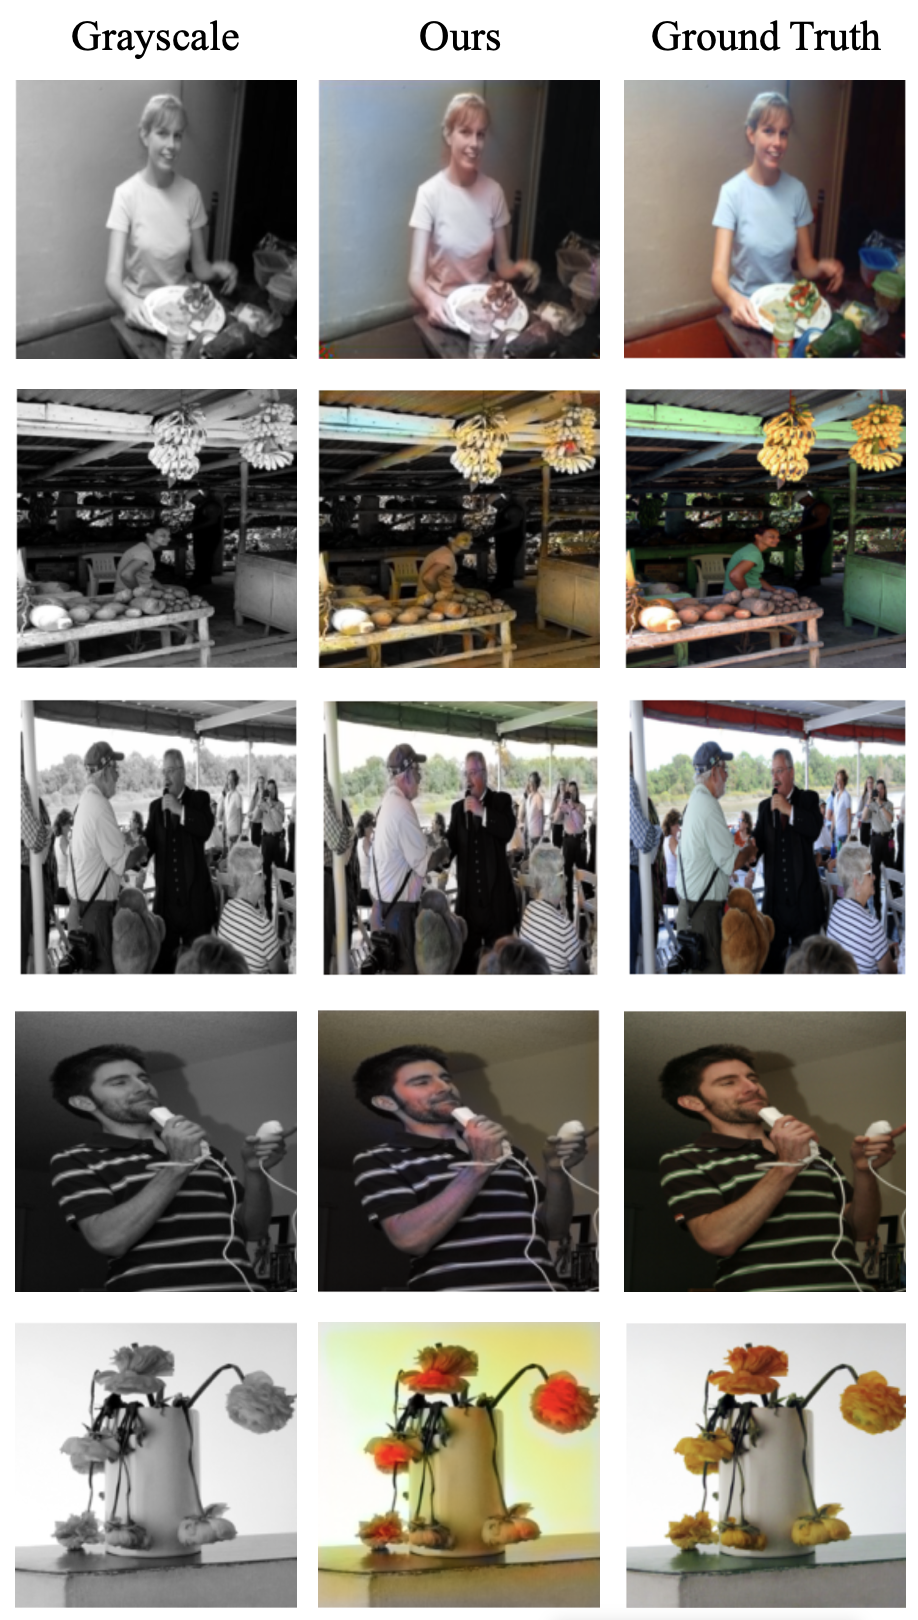
\includegraphics[width=1\linewidth]{latex/succesful colorizations.png}
    \caption{Succesful colorizations. (1) Succesful color ascription to clothing. (2) Semantic segmentation of bananas. (3 and 4) People. (5) Well colored flower, boundaries well respected. }
    \label{fig:enter-label}
\end{figure}


\subsection{Qualitative Evaluation of the Results}
Some examples from our test results on COCO can be found in Figures 4 and 5. We saved images from the test set of our last epoch and chose to display a variety of the most interesting results over different objects and settings. We found that batch 64 produced more accurate results, and that our model performed similarly to the pix2pix model, at times even creating more colorful outputs (see pizza on Figure 2). The trained generator produced brownish, dull outputs, showing that the adversarial training was an improvement on the simple CNN with Inception introduced by~\cite{Koalarization}. Pretraining considerably improved the quality of results. The addition of the COCO inception with semantic information at the beginning of the model seems to have improved the precision of the colorings. Both on the teddy bears and the pizza, the color in our model is well colored throughout the object, rather than just the center. 

Our model was exceptionally good at detecting and coloring human faces. It’s ascribed colors generally respected object boundaries. It was well capable of coloring natural objects such as the tree and the grass but still had some difficulty coloring objects with many possible colors such as clothing (with some exceptions, see Figure 5). The fact that the model colors some but not all clothing items suggest that it might yet be able to recognize them, suggesting that further training could fix the issue. The model excelled at coloring interiors, of which the COCO dataset had many examples and which generally do not have much variation in color, and often have many wooden elements. The colors images it generated were realistic but not necessarily close to the ground truth. Proving that adversarial training led the model to learn realistic colorings rather than just minimizing loss. The model's aptitude at identifying and coloring people is likely due to the class imbalance that characterizes the COCO dataset. Of the 80 classes it contains, "person" is by far the most common (Figure 6). This is a promising sign that the model would learn to colorize other objects well if trained on a larger dataset and for more epochs.
\begin{figure}
    \centering
    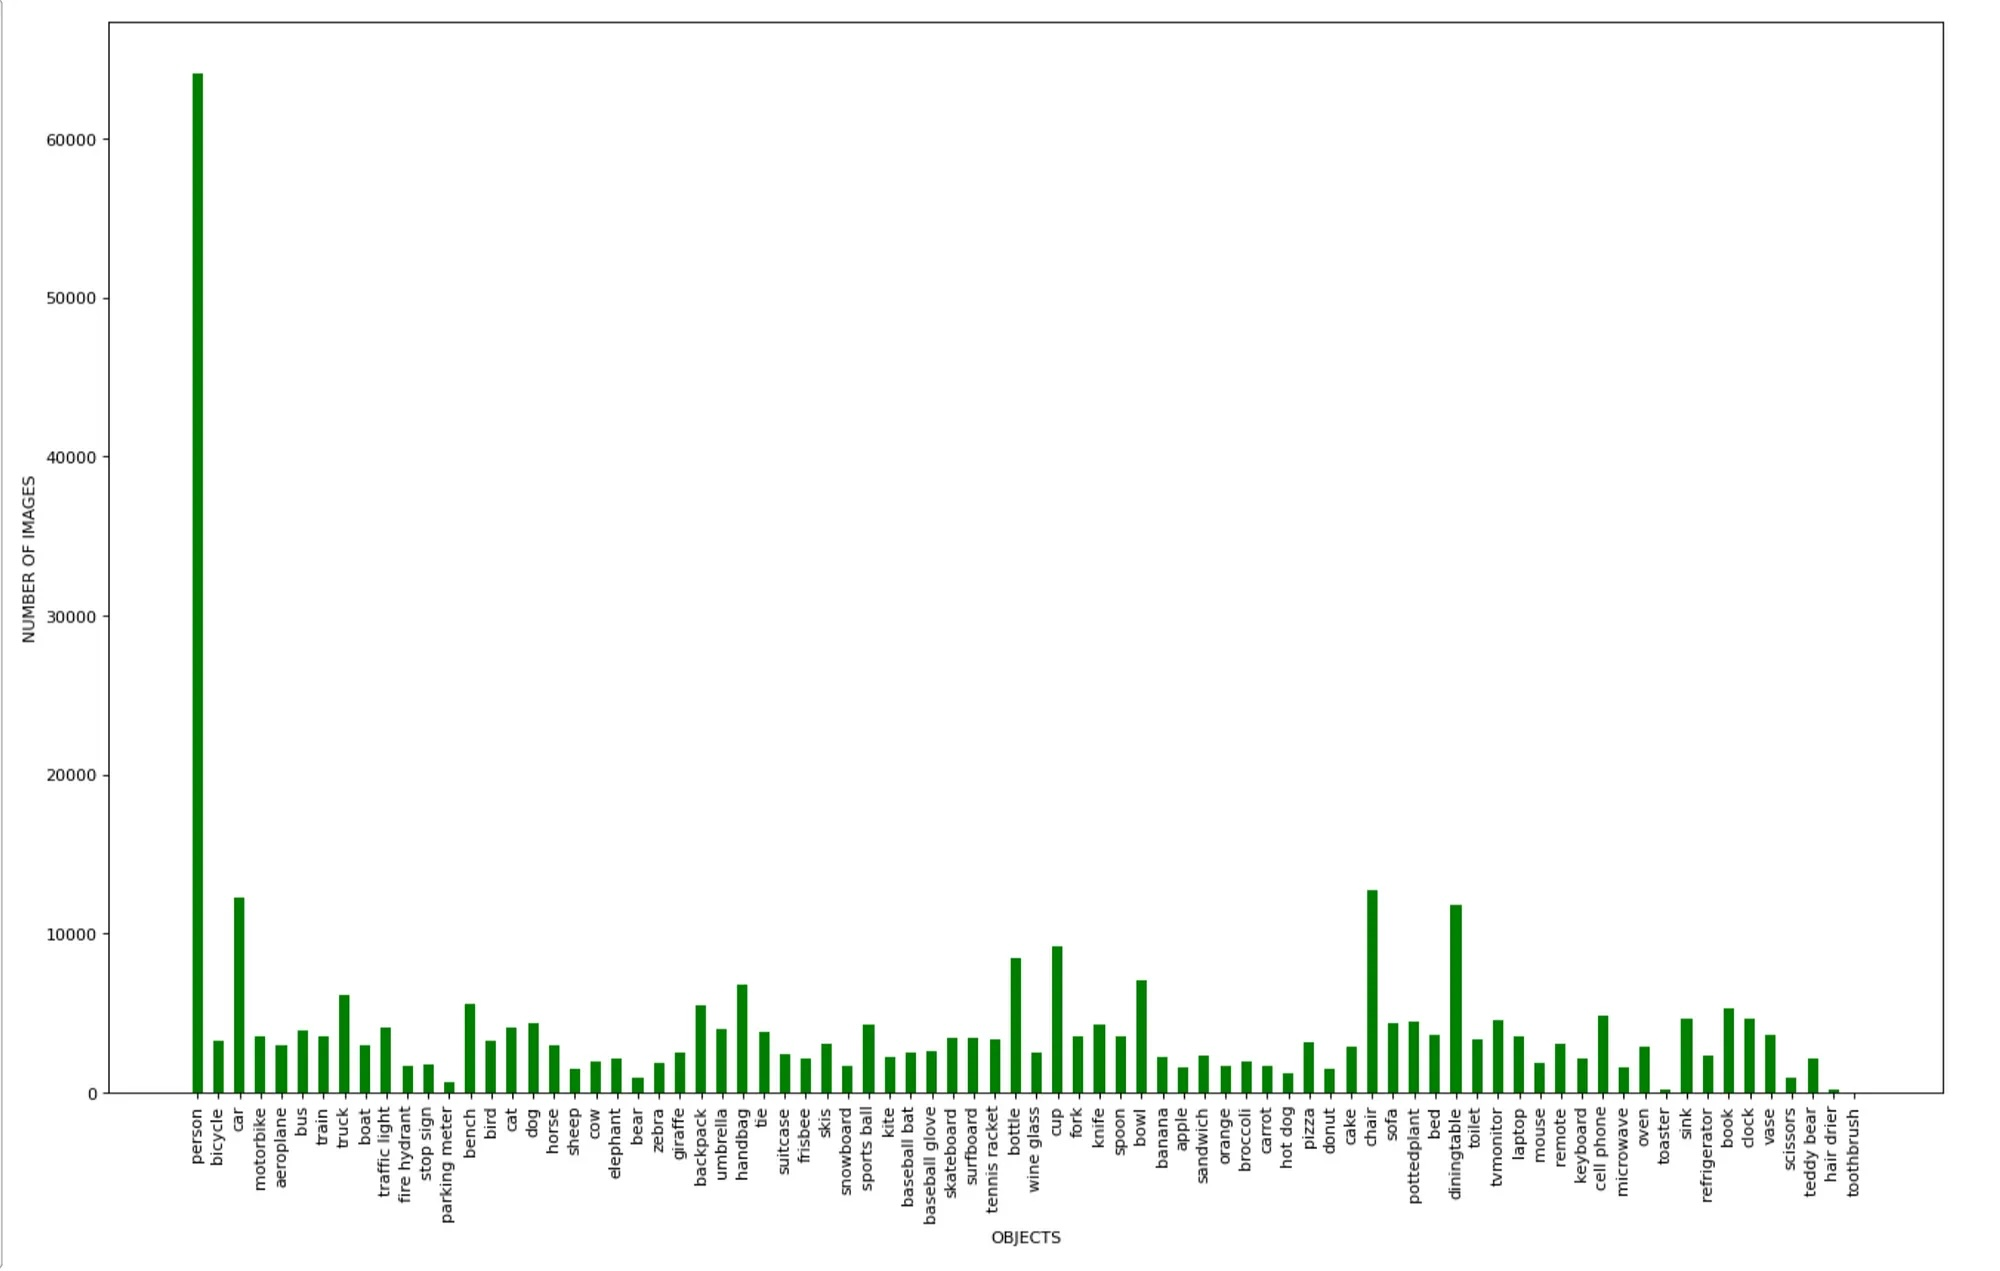
\includegraphics[width=0.5\linewidth]{latex/class_imbalance_coco.jpg}
    \caption{Class imbalance in the COCO dataset}
    \label{fig:enter-label}
\end{figure}


\subsection{Error Analysis}
\begin{figure}
    \centering
    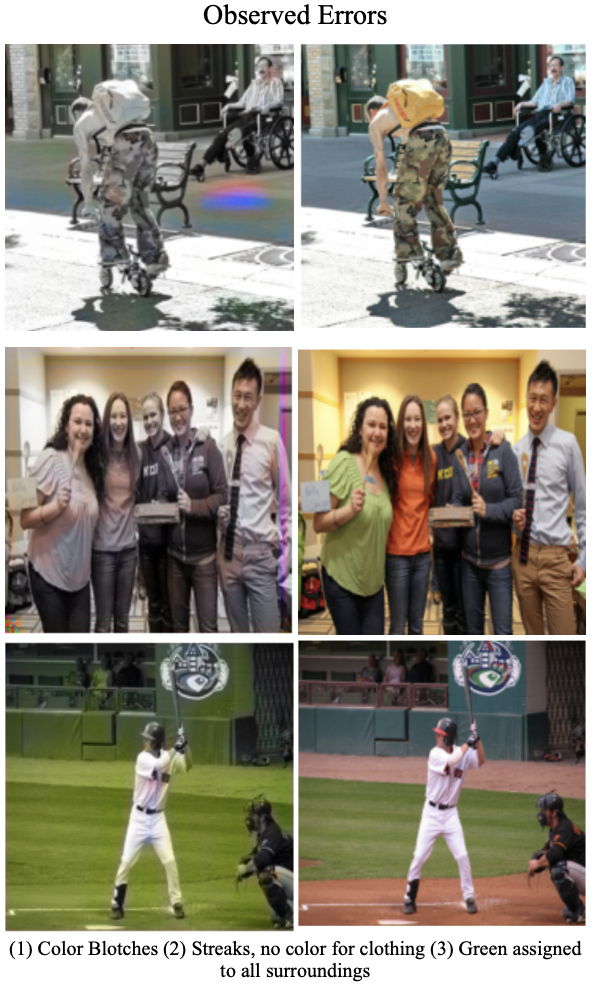
\includegraphics[width=0.5\linewidth]{common errors.png}
    \caption{Common Errors. (1) Color Blotches (2) Streaks, no color for clothing (3) Green assigned to all surroundings.}
    \label{fig:enter-label}
\end{figure}
Manual inspection of the model results on the test set provided us with insights on what the model was having difficulty with. Figure 4 shows a collection of failed colorizations. We can see that the GAN is still somewhat “shy” about coloring clothing items and often leaves this to be a gray and brownish color, with some exceptions. We found that during training, the model was able to ascribe color to areas where classifications model would have been less willing to. In Figure 8 we can see that in epoch 14 the road is colored green and man’s pants are colored blue. In epoch 15 the model corrects and leaves the image mostly gray. The model is still penalized for the unrealistic coloring, but the fact that on epoch 14 the model ascribed such strong colors suggests that it believes it can create realistic outputs with strong colorings and does not gray out images entirely, unlike classification models like "Deep Koalarization." We can also observe some streaks of “bleeding” in the images, colors that are not supposed to be there (for example the pink vertical line on Figure 7(2)) and some over-ascribed colors, such as the entirely green surroundings in 7(3). 

\begin{figure}
    \centering
    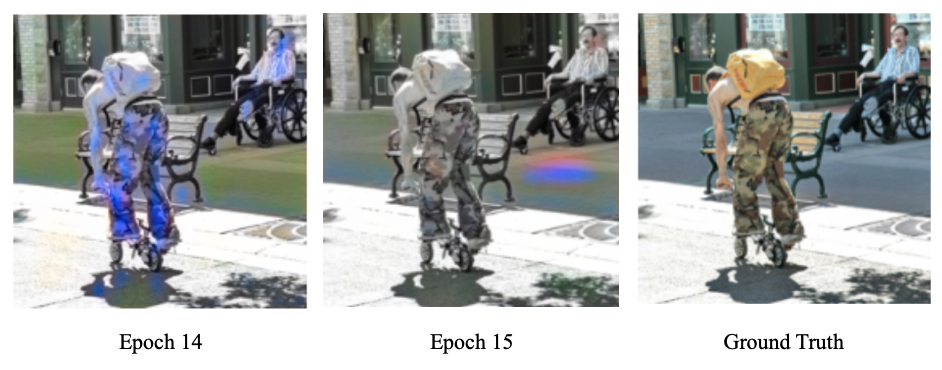
\includegraphics[width=0.5\linewidth]{epoch14_15.png}
    \caption{(1) Epoch 14 (2) Epoch 15. (3) Ground Truth. Model producing boldly colorized outputs at late iterations}
    \label{fig:enter-label}
\end{figure}

\subsection{Semantic information} 
From Figure 5(1) and 5(3) we can observe that our model has learnt semantic information. The models learned that grass and trees are green and that the bananas are yellow. It is also able to distinguish the background from buildings and objects. In our results we can also see that the model is able to recognize human faces and colors them with a beige, pinkish tone.It is even able to adequately color the pizza and teddy bears on Figure 4.  However, some objects like the clothing in Figure 7(2) and the furniture in 5(2) have not been learned and are left uncolored. We believe that training on a larger dataset, would allow our model to learn more objects and settings and their corresponding colors.
\begin{figure}
    \centering
    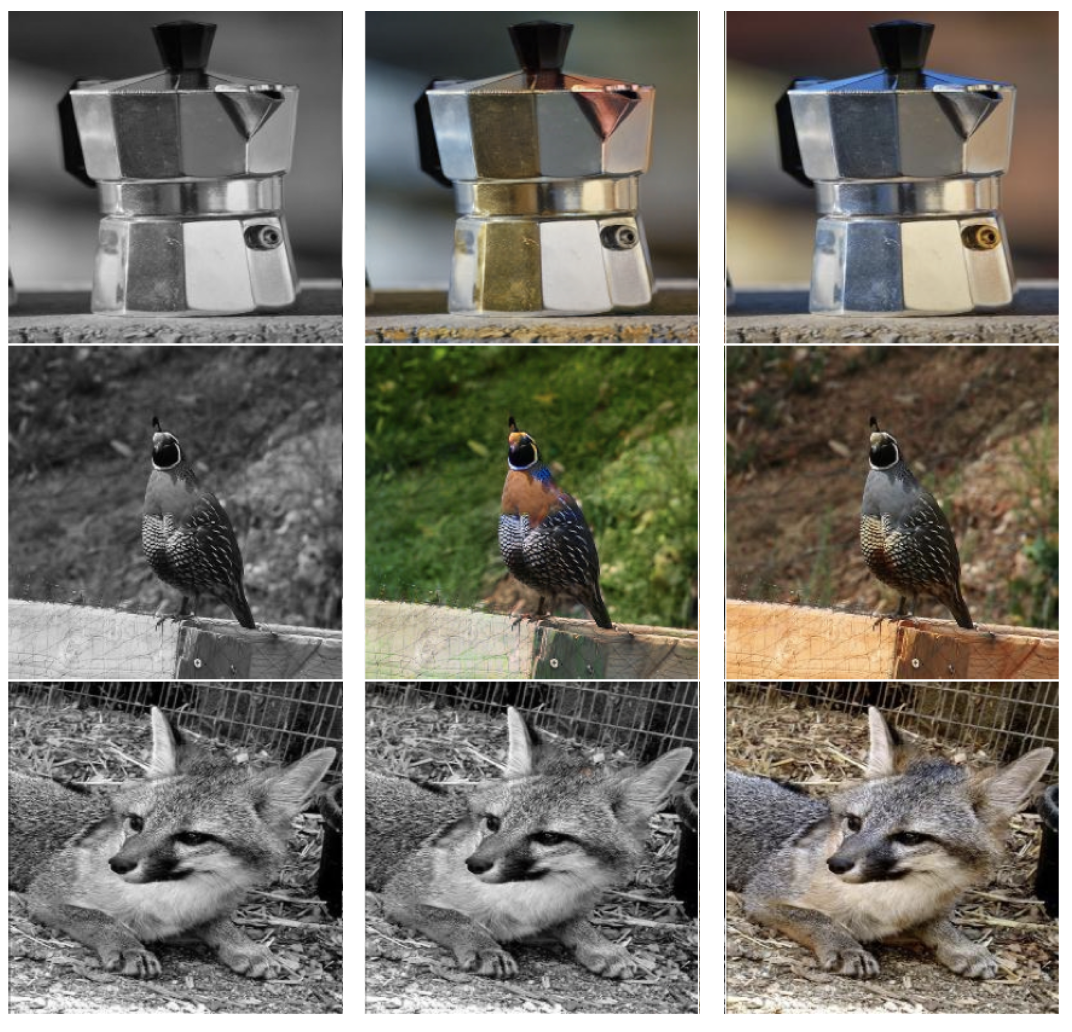
\includegraphics[width=0.5\linewidth]{pix2pix colorization.png}
    \caption{pix2pix colorization model trained on 1.2 million ImageNet images for 3 epochs `\cite{Pix2Pix}}
    \label{fig:enter-label}
\end{figure}

\subsection{Conclusion}
In this work, we compared the quantitative and qualitative results of colorization tasks using a GAN with a generator that incorporates semantic feature extraction via the Inception-ResNet-v2. For our experiments, we draw the following conclusions:
\begin{itemize}
    \item Our GAN produced convincing results when trained on 64 batches for 15 epochs with a pre-trained generator, showing that semantic feature extraction can be succesfully added to adversarially trained models.  It was particularly succesful at identifying and coloring people, which is an overrepresented class on the COCO data set. This suggests  that the model was effectively incorporating semantic segmentation as is also suggested by its ability to identify and color objects like bananas. These results also suggest that the model has the potential to perform well on a wide variety of objects if trained on a larger dataset. 
\end{itemize}
\begin{itemize}
    \item Our adversarially trained model performed much better than the pretrained generator with Inception-ResNet-v2 based on the model Baldassare et al. The adversarial training led to the model producing more colorful results that looked brighter and more realistic, whereas images generated by  Baldassare et al.'s model and the pretrained generator had much dimmer outputs caused by averaging the colors to minimize loss~\cite{Koalarization}. The adversarial training created mroe realistic results with brighter colors.
\end{itemize}
\begin{itemize}
    \item Our model performed convincing colorization and was only trained on 10,000 images for 15 epochs. The pix2pix colorization model was trained on 1.2 million training images for 3 epochs and produced highly-convincing colorization outputs (see Figure 9). Our model's high performance on its testing set with comparatively a lot less training data is a promising sign that it would produce even better results if similarly trained. Further research could compare the speed at which our model and  pix2pix trained on ImageNet achieve good results, as well as comparing the quality of the outputs.
\end{itemize}


{\small
\bibliographystyle{ieee}
\bibliography{egbib}
}

\section{Appendix}


\begin{table}
% 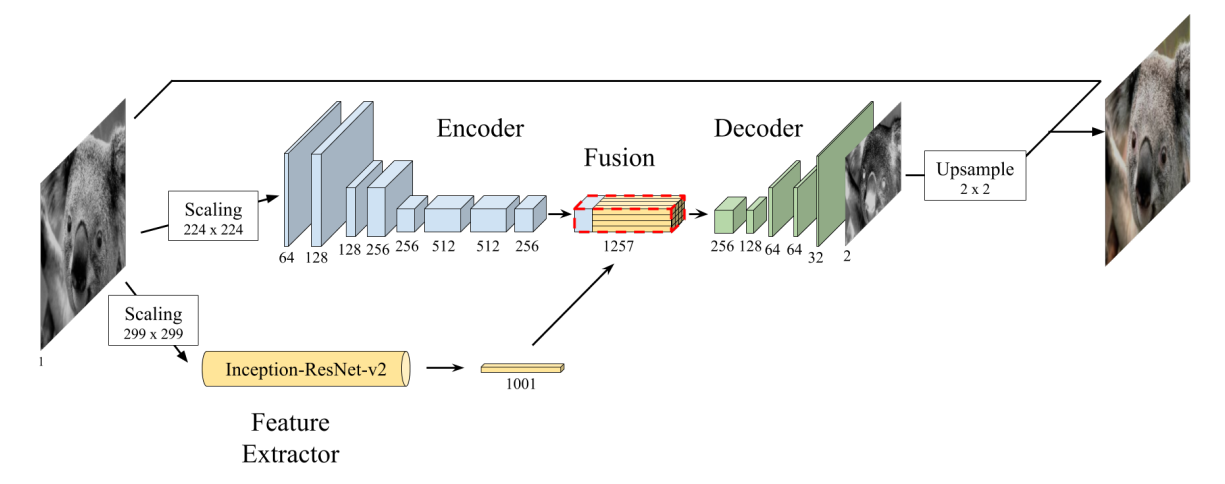
\includegraphics[width=5cm, height=4cm]{baldassare_model.png}
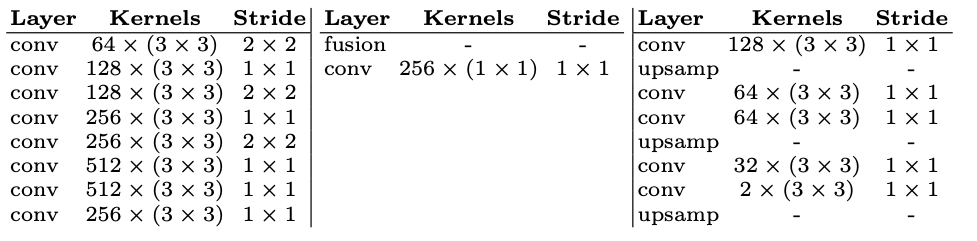
\includegraphics[width=1\linewidth]{Table.png}
\caption{An overview of the network architecture for the Baldassare et al. generator.}
\end{table}
\begin{figure}
    \centering
    \includegraphics{subdivision}
    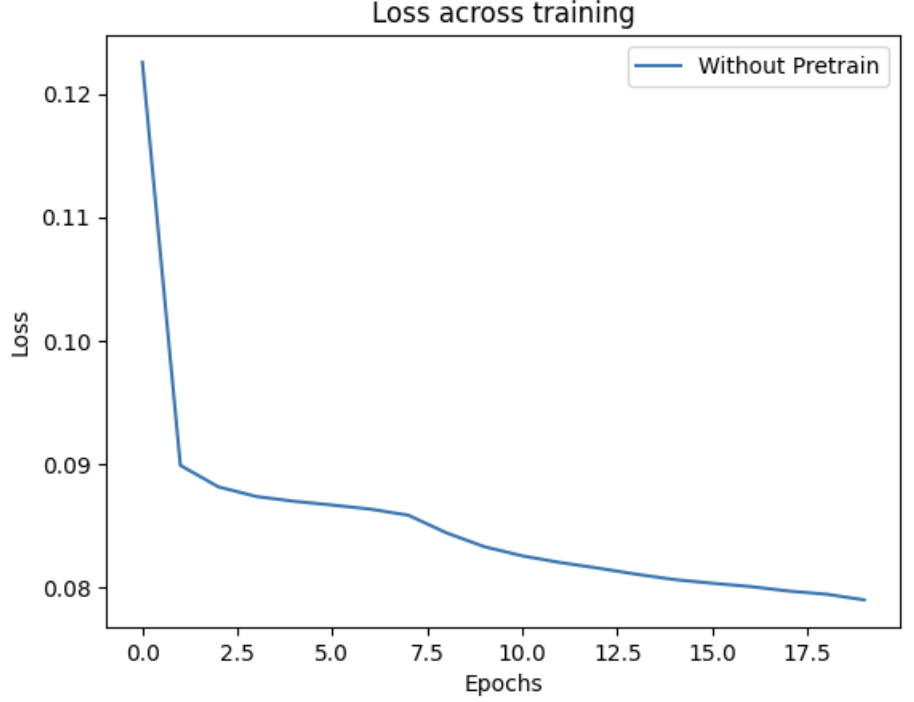
\includegraphics[width=0.5\linewidth]{pretraining loss.png}
    \caption{Training loss for during generator pretraining (20 epochs)}
    \label{fig:enter-label}
\end{figure}

\end{document}
